% Created by tikzDevice version 0.12.3.1 on 2021-12-10 10:16:37
% !TEX encoding = UTF-8 Unicode
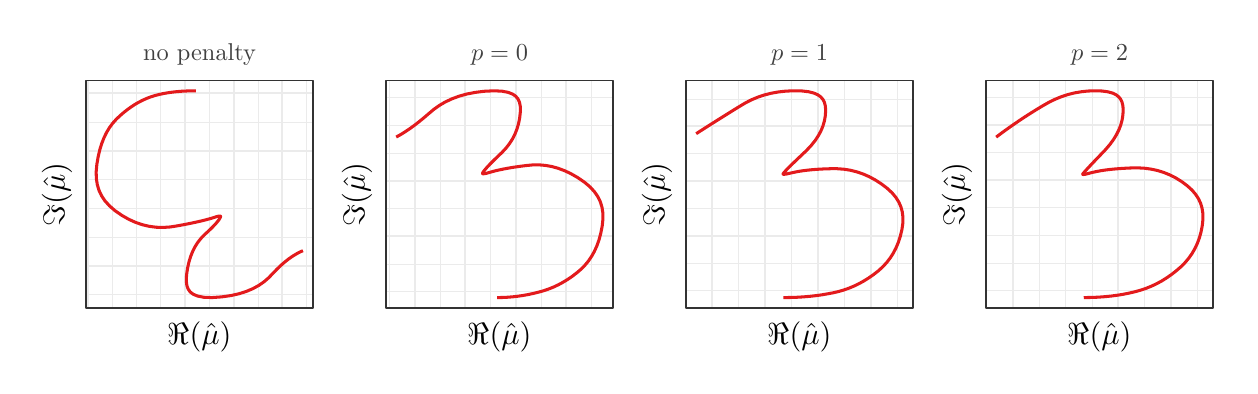
\begin{tikzpicture}[x=1pt,y=1pt]
\definecolor{fillColor}{RGB}{255,255,255}
\begin{scope}
\definecolor{drawColor}{RGB}{255,255,255}
\definecolor{fillColor}{RGB}{255,255,255}

\path[draw=drawColor,line width= 0.6pt,line join=round,line cap=round,fill=fillColor] ( -0.00, 11.43) rectangle (108.41,133.11);
\end{scope}
\begin{scope}
\definecolor{fillColor}{RGB}{255,255,255}

\path[fill=fillColor] ( 20.71, 32.15) rectangle (102.91,114.34);
\definecolor{drawColor}{gray}{0.92}

\path[draw=drawColor,line width= 0.3pt,line join=round] ( 20.71, 36.93) --
	(102.91, 36.93);

\path[draw=drawColor,line width= 0.3pt,line join=round] ( 20.71, 57.72) --
	(102.91, 57.72);

\path[draw=drawColor,line width= 0.3pt,line join=round] ( 20.71, 78.51) --
	(102.91, 78.51);

\path[draw=drawColor,line width= 0.3pt,line join=round] ( 20.71, 99.29) --
	(102.91, 99.29);

\path[draw=drawColor,line width= 0.3pt,line join=round] ( 30.22, 32.15) --
	( 30.22,114.34);

\path[draw=drawColor,line width= 0.3pt,line join=round] ( 47.79, 32.15) --
	( 47.79,114.34);

\path[draw=drawColor,line width= 0.3pt,line join=round] ( 65.36, 32.15) --
	( 65.36,114.34);

\path[draw=drawColor,line width= 0.3pt,line join=round] ( 82.93, 32.15) --
	( 82.93,114.34);

\path[draw=drawColor,line width= 0.3pt,line join=round] (100.50, 32.15) --
	(100.50,114.34);

\path[draw=drawColor,line width= 0.6pt,line join=round] ( 20.71, 47.33) --
	(102.91, 47.33);

\path[draw=drawColor,line width= 0.6pt,line join=round] ( 20.71, 68.11) --
	(102.91, 68.11);

\path[draw=drawColor,line width= 0.6pt,line join=round] ( 20.71, 88.90) --
	(102.91, 88.90);

\path[draw=drawColor,line width= 0.6pt,line join=round] ( 20.71,109.69) --
	(102.91,109.69);

\path[draw=drawColor,line width= 0.6pt,line join=round] ( 21.44, 32.15) --
	( 21.44,114.34);

\path[draw=drawColor,line width= 0.6pt,line join=round] ( 39.01, 32.15) --
	( 39.01,114.34);

\path[draw=drawColor,line width= 0.6pt,line join=round] ( 56.57, 32.15) --
	( 56.57,114.34);

\path[draw=drawColor,line width= 0.6pt,line join=round] ( 74.14, 32.15) --
	( 74.14,114.34);

\path[draw=drawColor,line width= 0.6pt,line join=round] ( 91.71, 32.15) --
	( 91.71,114.34);
\definecolor{drawColor}{RGB}{227,26,28}

\path[draw=drawColor,line width= 1.1pt,line join=round] ( 60.45,110.60) --
	( 57.80,110.56) --
	( 55.34,110.44) --
	( 53.07,110.24) --
	( 50.96,109.98) --
	( 49.02,109.66) --
	( 47.23,109.28) --
	( 45.59,108.85) --
	( 44.08,108.37) --
	( 42.67,107.83) --
	( 41.29,107.21) --
	( 39.91,106.51) --
	( 38.54,105.72) --
	( 37.17,104.83) --
	( 35.80,103.85) --
	( 34.42,102.77) --
	( 33.05,101.58) --
	( 31.68,100.28) --
	( 30.41, 98.85) --
	( 29.26, 97.30) --
	( 28.23, 95.59) --
	( 27.31, 93.71) --
	( 26.49, 91.64) --
	( 25.78, 89.36) --
	( 25.18, 86.84) --
	( 24.70, 84.05) --
	( 24.45, 81.29) --
	( 24.52, 78.84) --
	( 24.87, 76.63) --
	( 25.49, 74.59) --
	( 26.40, 72.67) --
	( 27.64, 70.82) --
	( 29.26, 69.02) --
	( 31.32, 67.24) --
	( 33.78, 65.56) --
	( 36.24, 64.16) --
	( 38.68, 63.05) --
	( 41.13, 62.21) --
	( 43.60, 61.63) --
	( 46.10, 61.30) --
	( 48.65, 61.22) --
	( 51.28, 61.40) --
	( 53.98, 61.83) --
	( 56.49, 62.30) --
	( 58.74, 62.75) --
	( 60.73, 63.18) --
	( 62.49, 63.58) --
	( 64.04, 63.97) --
	( 65.37, 64.33) --
	( 66.52, 64.66) --
	( 67.50, 64.98) --
	( 68.25, 65.21) --
	( 68.76, 65.32) --
	( 69.09, 65.35) --
	( 69.27, 65.33) --
	( 69.35, 65.28) --
	( 69.39, 65.20) --
	( 69.39, 65.08) --
	( 69.32, 64.88) --
	( 69.15, 64.55) --
	( 68.91, 64.15) --
	( 68.56, 63.66) --
	( 68.09, 63.08) --
	( 67.49, 62.39) --
	( 66.73, 61.59) --
	( 65.81, 60.66) --
	( 64.69, 59.60) --
	( 63.39, 58.41) --
	( 62.17, 57.10) --
	( 61.08, 55.69) --
	( 60.12, 54.16) --
	( 59.29, 52.50) --
	( 58.57, 50.68) --
	( 57.96, 48.69) --
	( 57.48, 46.50) --
	( 57.11, 44.09) --
	( 57.01, 41.88) --
	( 57.23, 40.21) --
	( 57.70, 38.93) --
	( 58.44, 37.91) --
	( 59.53, 37.08) --
	( 61.08, 36.43) --
	( 63.26, 36.00) --
	( 66.23, 35.88) --
	( 69.83, 36.13) --
	( 73.13, 36.60) --
	( 76.09, 37.27) --
	( 78.74, 38.11) --
	( 81.10, 39.12) --
	( 83.22, 40.28) --
	( 85.12, 41.60) --
	( 86.83, 43.08) --
	( 88.37, 44.70) --
	( 89.85, 46.22) --
	( 91.28, 47.58) --
	( 92.67, 48.79) --
	( 94.03, 49.85) --
	( 95.36, 50.78) --
	( 96.65, 51.58) --
	( 97.92, 52.27) --
	( 99.17, 52.83);
\definecolor{drawColor}{gray}{0.20}

\path[draw=drawColor,line width= 0.6pt,line join=round,line cap=round] ( 20.71, 32.15) rectangle (102.91,114.34);
\end{scope}
\begin{scope}
\definecolor{drawColor}{RGB}{0,0,0}

\node[text=drawColor,anchor=base,inner sep=0pt, outer sep=0pt, scale=  1.10] at ( 61.81, 19.07) {$\Re(\hat\mu)$};
\end{scope}
\begin{scope}
\definecolor{drawColor}{RGB}{0,0,0}

\node[text=drawColor,rotate= 90.00,anchor=base,inner sep=0pt, outer sep=0pt, scale=  1.10] at ( 13.08, 73.24) {$\Im(\hat\mu)$};
\end{scope}
\begin{scope}
\definecolor{drawColor}{gray}{0.25}

\node[text=drawColor,anchor=base,inner sep=0pt, outer sep=0pt, scale=  0.88] at ( 61.81,121.55) {no penalty};
\end{scope}
\begin{scope}
\definecolor{drawColor}{RGB}{255,255,255}
\definecolor{fillColor}{RGB}{255,255,255}

\path[draw=drawColor,line width= 0.6pt,line join=round,line cap=round,fill=fillColor] (108.41, 11.43) rectangle (216.81,133.11);
\end{scope}
\begin{scope}
\definecolor{fillColor}{RGB}{255,255,255}

\path[fill=fillColor] (129.12, 32.15) rectangle (211.31,114.34);
\definecolor{drawColor}{gray}{0.92}

\path[draw=drawColor,line width= 0.3pt,line join=round] (129.12, 48.03) --
	(211.31, 48.03);

\path[draw=drawColor,line width= 0.3pt,line join=round] (129.12, 68.06) --
	(211.31, 68.06);

\path[draw=drawColor,line width= 0.3pt,line join=round] (129.12, 88.08) --
	(211.31, 88.08);

\path[draw=drawColor,line width= 0.3pt,line join=round] (129.12,108.11) --
	(211.31,108.11);

\path[draw=drawColor,line width= 0.3pt,line join=round] (130.43, 32.15) --
	(130.43,114.34);

\path[draw=drawColor,line width= 0.3pt,line join=round] (148.69, 32.15) --
	(148.69,114.34);

\path[draw=drawColor,line width= 0.3pt,line join=round] (166.94, 32.15) --
	(166.94,114.34);

\path[draw=drawColor,line width= 0.3pt,line join=round] (185.19, 32.15) --
	(185.19,114.34);

\path[draw=drawColor,line width= 0.3pt,line join=round] (203.44, 32.15) --
	(203.44,114.34);

\path[draw=drawColor,line width= 0.6pt,line join=round] (129.12, 38.02) --
	(211.31, 38.02);

\path[draw=drawColor,line width= 0.6pt,line join=round] (129.12, 58.04) --
	(211.31, 58.04);

\path[draw=drawColor,line width= 0.6pt,line join=round] (129.12, 78.07) --
	(211.31, 78.07);

\path[draw=drawColor,line width= 0.6pt,line join=round] (129.12, 98.09) --
	(211.31, 98.09);

\path[draw=drawColor,line width= 0.6pt,line join=round] (139.56, 32.15) --
	(139.56,114.34);

\path[draw=drawColor,line width= 0.6pt,line join=round] (157.81, 32.15) --
	(157.81,114.34);

\path[draw=drawColor,line width= 0.6pt,line join=round] (176.06, 32.15) --
	(176.06,114.34);

\path[draw=drawColor,line width= 0.6pt,line join=round] (194.32, 32.15) --
	(194.32,114.34);
\definecolor{drawColor}{RGB}{227,26,28}

\path[draw=drawColor,line width= 1.1pt,line join=round] (169.32, 35.88) --
	(171.20, 35.91) --
	(173.07, 36.00) --
	(174.94, 36.15) --
	(176.80, 36.37) --
	(178.67, 36.64) --
	(180.53, 36.97) --
	(182.40, 37.37) --
	(184.28, 37.83) --
	(186.14, 38.35) --
	(187.96, 38.98) --
	(189.73, 39.69) --
	(191.45, 40.50) --
	(193.14, 41.41) --
	(194.79, 42.41) --
	(196.42, 43.52) --
	(198.02, 44.74) --
	(199.58, 46.07) --
	(201.02, 47.51) --
	(202.31, 49.06) --
	(203.45, 50.74) --
	(204.47, 52.56) --
	(205.37, 54.54) --
	(206.14, 56.70) --
	(206.78, 59.07) --
	(207.30, 61.67) --
	(207.57, 64.23) --
	(207.53, 66.53) --
	(207.21, 68.61) --
	(206.60, 70.55) --
	(205.71, 72.38) --
	(204.49, 74.14) --
	(202.90, 75.88) --
	(200.86, 77.60) --
	(198.45, 79.24) --
	(196.06, 80.62) --
	(193.71, 81.73) --
	(191.39, 82.60) --
	(189.09, 83.23) --
	(186.79, 83.64) --
	(184.48, 83.84) --
	(182.13, 83.81) --
	(179.75, 83.58) --
	(177.50, 83.29) --
	(175.43, 82.99) --
	(173.54, 82.68) --
	(171.81, 82.36) --
	(170.24, 82.04) --
	(168.82, 81.71) --
	(167.54, 81.38) --
	(166.39, 81.05) --
	(165.47, 80.79) --
	(164.83, 80.65) --
	(164.43, 80.61) --
	(164.21, 80.62) --
	(164.10, 80.66) --
	(164.06, 80.71) --
	(164.06, 80.81) --
	(164.13, 80.98) --
	(164.30, 81.25) --
	(164.57, 81.63) --
	(164.96, 82.12) --
	(165.49, 82.74) --
	(166.19, 83.51) --
	(167.09, 84.44) --
	(168.20, 85.55) --
	(169.55, 86.86) --
	(171.13, 88.36) --
	(172.59, 89.94) --
	(173.84, 91.56) --
	(174.91, 93.24) --
	(175.79, 94.98) --
	(176.51, 96.80) --
	(177.07, 98.73) --
	(177.48,100.77) --
	(177.72,102.95) --
	(177.71,104.94) --
	(177.41,106.47) --
	(176.87,107.66) --
	(176.07,108.62) --
	(174.93,109.41) --
	(173.34,110.03) --
	(171.16,110.45) --
	(168.25,110.60) --
	(164.74,110.43) --
	(161.45,110.03) --
	(158.42,109.44) --
	(155.63,108.67) --
	(153.06,107.72) --
	(150.68,106.61) --
	(148.47,105.32) --
	(146.41,103.85) --
	(144.49,102.23) --
	(142.68,100.69) --
	(140.98, 99.31) --
	(139.39, 98.08) --
	(137.90, 97.00) --
	(136.50, 96.05) --
	(135.20, 95.22) --
	(133.99, 94.50) --
	(132.86, 93.90);
\definecolor{drawColor}{gray}{0.20}

\path[draw=drawColor,line width= 0.6pt,line join=round,line cap=round] (129.12, 32.15) rectangle (211.31,114.34);
\end{scope}
\begin{scope}
\definecolor{drawColor}{RGB}{0,0,0}

\node[text=drawColor,anchor=base,inner sep=0pt, outer sep=0pt, scale=  1.10] at (170.21, 19.07) {$\Re(\hat\mu)$};
\end{scope}
\begin{scope}
\definecolor{drawColor}{RGB}{0,0,0}

\node[text=drawColor,rotate= 90.00,anchor=base,inner sep=0pt, outer sep=0pt, scale=  1.10] at (121.48, 73.24) {$\Im(\hat\mu)$};
\end{scope}
\begin{scope}
\definecolor{drawColor}{gray}{0.25}

\node[text=drawColor,anchor=base,inner sep=0pt, outer sep=0pt, scale=  0.88] at (170.21,121.55) {$p = 0$};
\end{scope}
\begin{scope}
\definecolor{drawColor}{RGB}{255,255,255}
\definecolor{fillColor}{RGB}{255,255,255}

\path[draw=drawColor,line width= 0.6pt,line join=round,line cap=round,fill=fillColor] (216.81, 11.43) rectangle (325.22,133.11);
\end{scope}
\begin{scope}
\definecolor{fillColor}{RGB}{255,255,255}

\path[fill=fillColor] (237.52, 32.15) rectangle (319.72,114.34);
\definecolor{drawColor}{gray}{0.92}

\path[draw=drawColor,line width= 0.3pt,line join=round] (237.52, 48.27) --
	(319.71, 48.27);

\path[draw=drawColor,line width= 0.3pt,line join=round] (237.52, 68.07) --
	(319.71, 68.07);

\path[draw=drawColor,line width= 0.3pt,line join=round] (237.52, 87.86) --
	(319.71, 87.86);

\path[draw=drawColor,line width= 0.3pt,line join=round] (237.52,107.66) --
	(319.71,107.66);

\path[draw=drawColor,line width= 0.3pt,line join=round] (256.51, 32.15) --
	(256.51,114.34);

\path[draw=drawColor,line width= 0.3pt,line join=round] (275.64, 32.15) --
	(275.64,114.34);

\path[draw=drawColor,line width= 0.3pt,line join=round] (294.78, 32.15) --
	(294.78,114.34);

\path[draw=drawColor,line width= 0.3pt,line join=round] (313.91, 32.15) --
	(313.91,114.34);

\path[draw=drawColor,line width= 0.6pt,line join=round] (237.52, 38.38) --
	(319.71, 38.38);

\path[draw=drawColor,line width= 0.6pt,line join=round] (237.52, 58.17) --
	(319.71, 58.17);

\path[draw=drawColor,line width= 0.6pt,line join=round] (237.52, 77.97) --
	(319.71, 77.97);

\path[draw=drawColor,line width= 0.6pt,line join=round] (237.52, 97.76) --
	(319.71, 97.76);

\path[draw=drawColor,line width= 0.6pt,line join=round] (246.94, 32.15) --
	(246.94,114.34);

\path[draw=drawColor,line width= 0.6pt,line join=round] (266.07, 32.15) --
	(266.07,114.34);

\path[draw=drawColor,line width= 0.6pt,line join=round] (285.21, 32.15) --
	(285.21,114.34);

\path[draw=drawColor,line width= 0.6pt,line join=round] (304.34, 32.15) --
	(304.34,114.34);
\definecolor{drawColor}{RGB}{227,26,28}

\path[draw=drawColor,line width= 1.1pt,line join=round] (272.78, 35.88) --
	(275.24, 35.91) --
	(277.63, 35.99) --
	(279.95, 36.13) --
	(282.20, 36.32) --
	(284.39, 36.56) --
	(286.52, 36.85) --
	(288.59, 37.20) --
	(290.61, 37.58) --
	(292.57, 38.03) --
	(294.49, 38.58) --
	(296.37, 39.24) --
	(298.21, 40.00) --
	(300.03, 40.87) --
	(301.82, 41.86) --
	(303.60, 42.97) --
	(305.36, 44.20) --
	(307.10, 45.55) --
	(308.69, 47.01) --
	(310.11, 48.55) --
	(311.38, 50.20) --
	(312.50, 51.95) --
	(313.47, 53.83) --
	(314.32, 55.86) --
	(315.03, 58.05) --
	(315.60, 60.42) --
	(315.94, 62.77) --
	(315.98, 64.89) --
	(315.74, 66.83) --
	(315.25, 68.65) --
	(314.48, 70.39) --
	(313.42, 72.08) --
	(312.02, 73.75) --
	(310.22, 75.41) --
	(308.08, 77.03) --
	(305.92, 78.42) --
	(303.74, 79.59) --
	(301.54, 80.55) --
	(299.31, 81.31) --
	(297.03, 81.88) --
	(294.68, 82.26) --
	(292.25, 82.44) --
	(289.74, 82.44) --
	(287.36, 82.36) --
	(285.15, 82.24) --
	(283.12, 82.08) --
	(281.26, 81.89) --
	(279.55, 81.67) --
	(277.99, 81.42) --
	(276.58, 81.14) --
	(275.29, 80.85) --
	(274.25, 80.61) --
	(273.54, 80.48) --
	(273.08, 80.43) --
	(272.82, 80.43) --
	(272.70, 80.47) --
	(272.66, 80.51) --
	(272.66, 80.57) --
	(272.72, 80.70) --
	(272.88, 80.91) --
	(273.17, 81.25) --
	(273.60, 81.72) --
	(274.21, 82.36) --
	(275.03, 83.19) --
	(276.09, 84.24) --
	(277.43, 85.53) --
	(279.07, 87.08) --
	(281.00, 88.91) --
	(282.76, 90.76) --
	(284.22, 92.58) --
	(285.40, 94.36) --
	(286.35, 96.13) --
	(287.07, 97.89) --
	(287.59, 99.67) --
	(287.91,101.48) --
	(288.05,103.35) --
	(287.95,105.04) --
	(287.61,106.39) --
	(287.06,107.48) --
	(286.29,108.38) --
	(285.23,109.14) --
	(283.81,109.77) --
	(281.93,110.25) --
	(279.46,110.54) --
	(276.51,110.60) --
	(273.66,110.48) --
	(270.97,110.18) --
	(268.40,109.72) --
	(265.94,109.10) --
	(263.59,108.32) --
	(261.32,107.38) --
	(259.13,106.27) --
	(257.01,105.01) --
	(254.92,103.72) --
	(252.87,102.44) --
	(250.85,101.18) --
	(248.87, 99.94) --
	(246.92, 98.71) --
	(245.00, 97.49) --
	(243.11, 96.29) --
	(241.26, 95.10);
\definecolor{drawColor}{gray}{0.20}

\path[draw=drawColor,line width= 0.6pt,line join=round,line cap=round] (237.52, 32.15) rectangle (319.72,114.34);
\end{scope}
\begin{scope}
\definecolor{drawColor}{RGB}{0,0,0}

\node[text=drawColor,anchor=base,inner sep=0pt, outer sep=0pt, scale=  1.10] at (278.62, 19.07) {$\Re(\hat\mu)$};
\end{scope}
\begin{scope}
\definecolor{drawColor}{RGB}{0,0,0}

\node[text=drawColor,rotate= 90.00,anchor=base,inner sep=0pt, outer sep=0pt, scale=  1.10] at (229.89, 73.24) {$\Im(\hat\mu)$};
\end{scope}
\begin{scope}
\definecolor{drawColor}{gray}{0.25}

\node[text=drawColor,anchor=base,inner sep=0pt, outer sep=0pt, scale=  0.88] at (278.62,121.55) {$p = 1$};
\end{scope}
\begin{scope}
\definecolor{drawColor}{RGB}{255,255,255}
\definecolor{fillColor}{RGB}{255,255,255}

\path[draw=drawColor,line width= 0.6pt,line join=round,line cap=round,fill=fillColor] (325.21, 11.43) rectangle (433.62,133.11);
\end{scope}
\begin{scope}
\definecolor{fillColor}{RGB}{255,255,255}

\path[fill=fillColor] (345.93, 32.15) rectangle (428.12,114.34);
\definecolor{drawColor}{gray}{0.92}

\path[draw=drawColor,line width= 0.3pt,line join=round] (345.93, 48.37) --
	(428.12, 48.37);

\path[draw=drawColor,line width= 0.3pt,line join=round] (345.93, 68.35) --
	(428.12, 68.35);

\path[draw=drawColor,line width= 0.3pt,line join=round] (345.93, 88.34) --
	(428.12, 88.34);

\path[draw=drawColor,line width= 0.3pt,line join=round] (345.93,108.33) --
	(428.12,108.33);

\path[draw=drawColor,line width= 0.3pt,line join=round] (346.28, 32.15) --
	(346.28,114.34);

\path[draw=drawColor,line width= 0.3pt,line join=round] (365.27, 32.15) --
	(365.27,114.34);

\path[draw=drawColor,line width= 0.3pt,line join=round] (384.27, 32.15) --
	(384.27,114.34);

\path[draw=drawColor,line width= 0.3pt,line join=round] (403.26, 32.15) --
	(403.26,114.34);

\path[draw=drawColor,line width= 0.3pt,line join=round] (422.25, 32.15) --
	(422.25,114.34);

\path[draw=drawColor,line width= 0.6pt,line join=round] (345.93, 38.38) --
	(428.12, 38.38);

\path[draw=drawColor,line width= 0.6pt,line join=round] (345.93, 58.36) --
	(428.12, 58.36);

\path[draw=drawColor,line width= 0.6pt,line join=round] (345.93, 78.35) --
	(428.12, 78.35);

\path[draw=drawColor,line width= 0.6pt,line join=round] (345.93, 98.33) --
	(428.12, 98.33);

\path[draw=drawColor,line width= 0.6pt,line join=round] (355.78, 32.15) --
	(355.78,114.34);

\path[draw=drawColor,line width= 0.6pt,line join=round] (374.77, 32.15) --
	(374.77,114.34);

\path[draw=drawColor,line width= 0.6pt,line join=round] (393.76, 32.15) --
	(393.76,114.34);

\path[draw=drawColor,line width= 0.6pt,line join=round] (412.76, 32.15) --
	(412.76,114.34);
\definecolor{drawColor}{RGB}{227,26,28}

\path[draw=drawColor,line width= 1.1pt,line join=round] (381.31, 35.88) --
	(383.94, 35.92) --
	(386.47, 36.02) --
	(388.92, 36.20) --
	(391.28, 36.44) --
	(393.55, 36.74) --
	(395.75, 37.11) --
	(397.87, 37.53) --
	(399.92, 38.01) --
	(401.90, 38.57) --
	(403.83, 39.22) --
	(405.71, 39.98) --
	(407.56, 40.85) --
	(409.37, 41.82) --
	(411.14, 42.92) --
	(412.90, 44.13) --
	(414.63, 45.47) --
	(416.33, 46.93) --
	(417.88, 48.48) --
	(419.24, 50.09) --
	(420.43, 51.79) --
	(421.47, 53.58) --
	(422.36, 55.47) --
	(423.10, 57.48) --
	(423.70, 59.64) --
	(424.15, 61.96) --
	(424.38, 64.23) --
	(424.35, 66.29) --
	(424.06, 68.18) --
	(423.54, 69.93) --
	(422.77, 71.59) --
	(421.73, 73.19) --
	(420.39, 74.76) --
	(418.68, 76.31) --
	(416.66, 77.81) --
	(414.59, 79.10) --
	(412.47, 80.18) --
	(410.29, 81.07) --
	(408.03, 81.78) --
	(405.69, 82.29) --
	(403.25, 82.62) --
	(400.68, 82.76) --
	(398.00, 82.70) --
	(395.46, 82.57) --
	(393.14, 82.40) --
	(391.04, 82.20) --
	(389.14, 81.97) --
	(387.42, 81.71) --
	(385.89, 81.42) --
	(384.52, 81.12) --
	(383.31, 80.81) --
	(382.34, 80.55) --
	(381.69, 80.41) --
	(381.28, 80.36) --
	(381.06, 80.36) --
	(380.96, 80.39) --
	(380.93, 80.43) --
	(380.94, 80.49) --
	(381.02, 80.63) --
	(381.21, 80.87) --
	(381.52, 81.23) --
	(381.97, 81.73) --
	(382.58, 82.41) --
	(383.39, 83.28) --
	(384.42, 84.38) --
	(385.70, 85.72) --
	(387.25, 87.33) --
	(389.06, 89.22) --
	(390.70, 91.13) --
	(392.06, 92.99) --
	(393.16, 94.79) --
	(394.04, 96.56) --
	(394.70, 98.31) --
	(395.17,100.06) --
	(395.45,101.82) --
	(395.56,103.61) --
	(395.45,105.24) --
	(395.13,106.53) --
	(394.63,107.58) --
	(393.92,108.44) --
	(392.98,109.17) --
	(391.72,109.77) --
	(390.06,110.23) --
	(387.90,110.52) --
	(385.31,110.60) --
	(382.77,110.51) --
	(380.31,110.24) --
	(377.90,109.82) --
	(375.55,109.23) --
	(373.24,108.47) --
	(370.96,107.54) --
	(368.70,106.44) --
	(366.45,105.16) --
	(364.23,103.82) --
	(362.05,102.46) --
	(359.90,101.08) --
	(357.79, 99.67) --
	(355.71, 98.25) --
	(353.66, 96.81) --
	(351.65, 95.35) --
	(349.67, 93.86);
\definecolor{drawColor}{gray}{0.20}

\path[draw=drawColor,line width= 0.6pt,line join=round,line cap=round] (345.93, 32.15) rectangle (428.12,114.34);
\end{scope}
\begin{scope}
\definecolor{drawColor}{RGB}{0,0,0}

\node[text=drawColor,anchor=base,inner sep=0pt, outer sep=0pt, scale=  1.10] at (387.02, 19.07) {$\Re(\hat\mu)$};
\end{scope}
\begin{scope}
\definecolor{drawColor}{RGB}{0,0,0}

\node[text=drawColor,rotate= 90.00,anchor=base,inner sep=0pt, outer sep=0pt, scale=  1.10] at (338.29, 73.24) {$\Im(\hat\mu)$};
\end{scope}
\begin{scope}
\definecolor{drawColor}{gray}{0.25}

\node[text=drawColor,anchor=base,inner sep=0pt, outer sep=0pt, scale=  0.88] at (387.02,121.55) {$p = 2$};
\end{scope}
\end{tikzpicture}
